\def\handout{0} %handout-version?

\ifnum\handout=0
	\documentclass{beamer}
\else
	\documentclass[handout]{beamer}
\fi
\usetheme{HUmetrics}
\usepackage{graphicx}
\usepackage{tabularx}
\usepackage[utf8]{inputenc}
\usepackage{listings}
\useinnertheme{HUmetrics}
\useoutertheme{HUmetrics}

\usepackage{tikz}
\usetikzlibrary{arrows, automata, decorations.pathreplacing}

\tikzset{
	brc/.style={
		decorate,
		decoration={
			brace,
			amplitude=1.5ex
		},
		thick
	}
}

\begin{document}
\title{Evolutionary swarm robotics}
\author{Frank Lange\\ Phillipp Schoppmann}
\date{12. Juni 2013}

\frame{\titlepage}

\section*{Outline}
\frame{\tableofcontents}

\section{Overview}
\frame{\tableofcontents[currentsection]}

\frame[<+->]{\frametitle{Swarm robotics}
\begin{itemize}
	\item robots cooperating to reach a certain goal
	\item decentralization of control
	\item limited communication abilities
	\item use of local information
	\item emergence of global behavior
\end{itemize}
\hfill \\[1ex]
\visible<+->{\begin{tabularx}{0.8\textwidth}{p{3em}X}
		\raggedleft $\Rightarrow$ & \emph{Although each robot is autonomous, the swarm can solve problems that a single robot can't.}
	\end{tabularx}
}}


\frame[<+->]{\frametitle{The Swarm Bot}
\only<+->{In this presentation, we will focus on a so-called \emph{Swarm Bot}, which is a swarm of \emph{S-Bots}}
\visible<+->{
\begin{center}
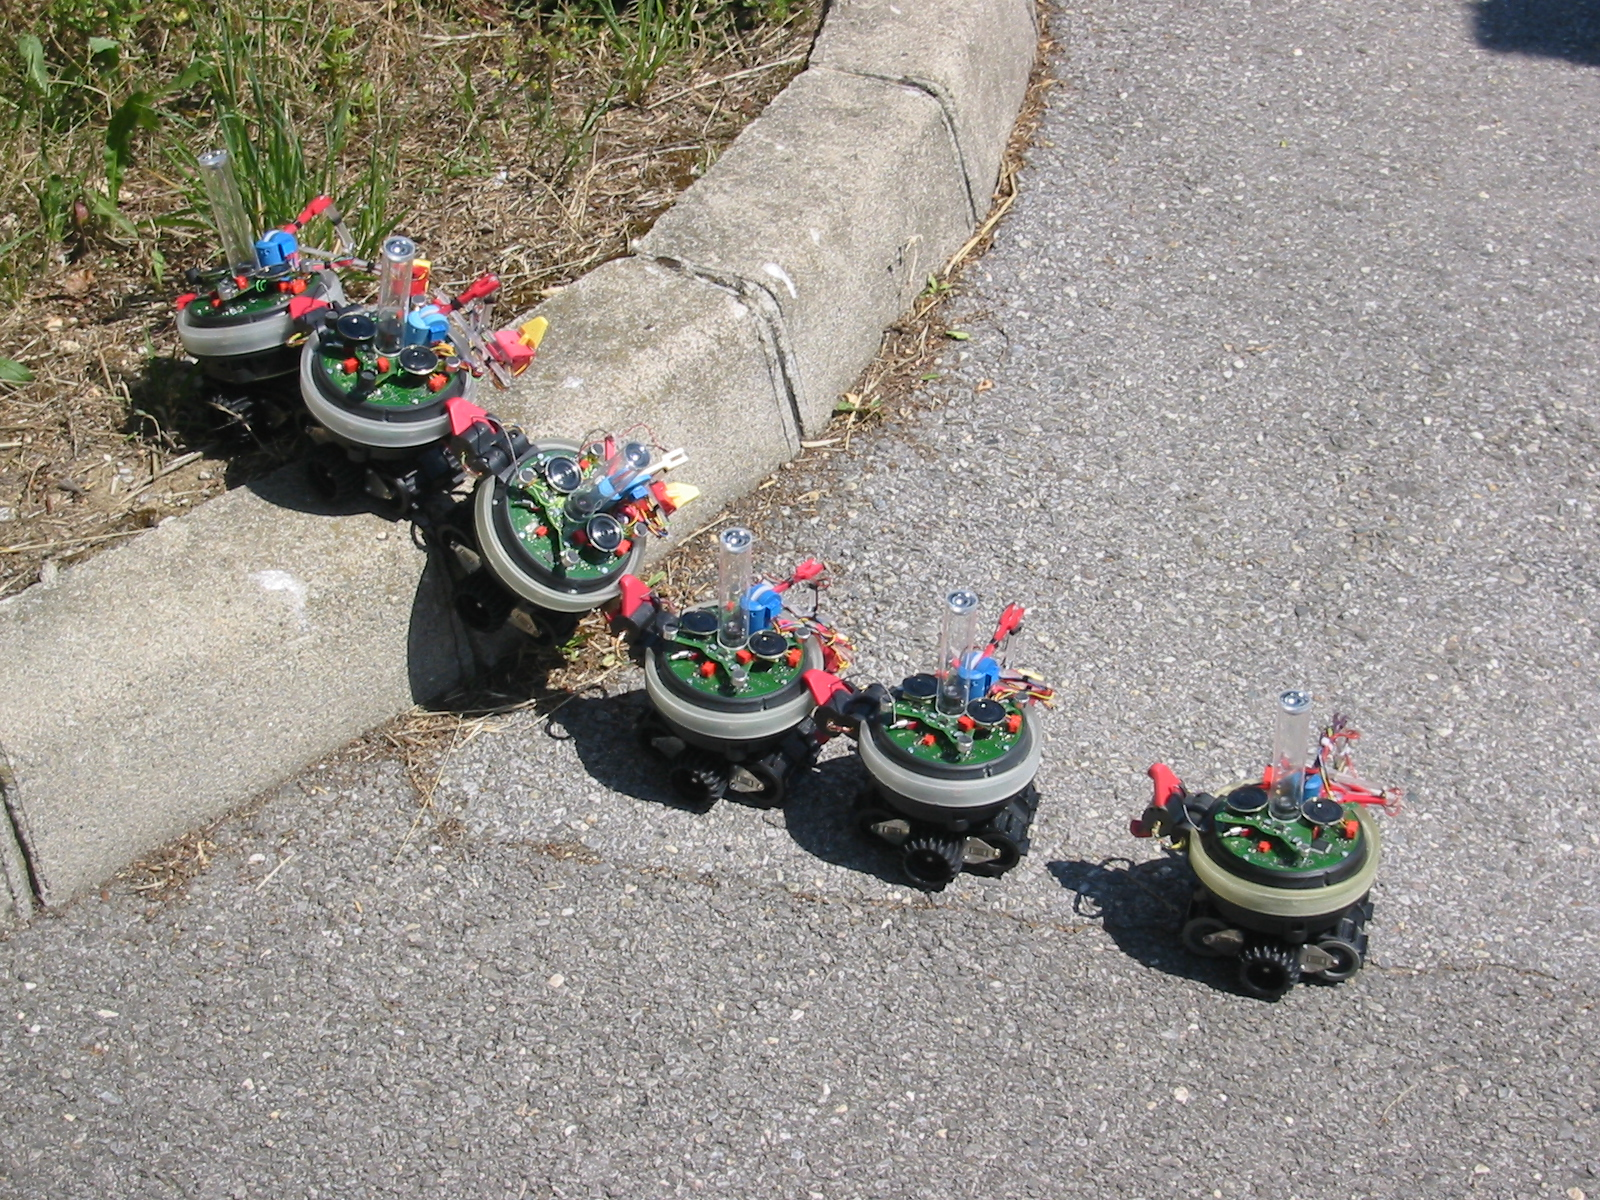
\includegraphics[
		width=\textwidth,
		height=0.6\textheight,
		keepaspectratio,
		clip,
		trim=0cm 4cm 0cm 4.5cm
	]{pics/sbots2.jpg}
\end{center}
}}

\frame[<+->]{\frametitle{S-Bots}
\only<+->{Mobile robots that can connect to/disconnect from each other}
\visible<+->{
\begin{center}
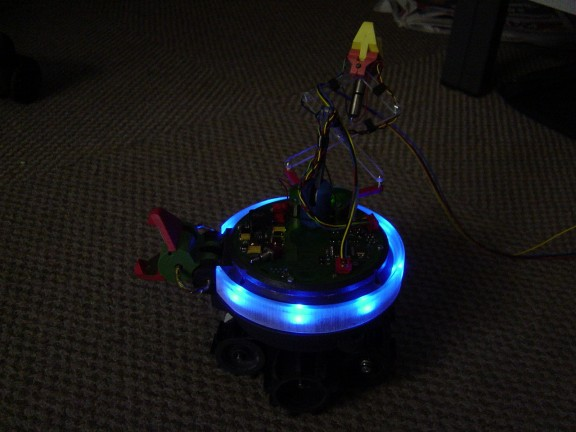
\includegraphics[
		width=\textwidth,
		height=0.6\textheight,
		keepaspectratio,
		clip,
	]{pics/sbots4.jpg}
\end{center}
}}

\section{Goal definition}
\frame{\tableofcontents[currentsection]}

\frame[<+->]{\frametitle{Tasks}
\begin{block}{Possible task for a Swarm Bot}
	\begin{itemize}
		\item move objects
		\item move through (tough) physical terrain
	\end{itemize}
\visible<+->{For some tasks however, acting as single S-Bots might be more efficient, like finding a goal location or determining an optimal path.}
\end{block}
\begin{block}{Focus of this presentation}
\begin{itemize}
	\item Aggregation
	\item Coordinated motion
\end{itemize}
\end{block}
}

\frame[<+->]{\frametitle{Self-organization}
\begin{itemize}
	\item system changes from a disordered to an ordered state using only local interactions
	\item uses positive/negative feedback
	\item Positive feedback:
	\begin{itemize}
		\item amplification of some property that emerges from random interactions (snow ball effect)
		\item increases exponentially over time
	\end{itemize}
	\item Negative feedback:
	\begin{itemize}
		\item regulation that often gets triggered by positive feedback exhausting some resource
	\end{itemize}
	\item Positive and negative feedback interact, keeping the system in a stable state.
\end{itemize}
}

\frame[<+->]{\frametitle{Problem}
\begin{itemize}
	\item Given a set of individual behaviors, it is difficult to predict the behavior that is going to emerge on a system level.
	\item Given a global behavior, it is difficult to decompose individual behaviors.
\end{itemize}
}

\frame[<+->]{\frametitle{Possible solution}
\begin{block}{Artificial Evolution}
	\begin{itemize}
		\item bypasses decomposing the rules/mechanisms for the target behavior (which may not even be possible)
		\item relies on the evaluation of the system as a whole
		\item can deal with the richness/complexity of the dynamic system, involving not only a multiple-agent scenario but also a possible physical link between the agents
		\item is easy to implement
	\end{itemize}
\end{block}
}

\frame[<+->]{\frametitle{How can we use this for our Swarm Bot?}
\pause
\begin{itemize}
	\item connect sensory input and motor output through an artificial neural network
	\item determine the details of this network using artificial evolution
\end{itemize}
}

\section{Used techniques}
\subsection{Artificial neural networks}
\frame{\tableofcontents[currentsection, currentsubsection]}

\frame[<+->]{\frametitle{Single Layer Perceptron}
\begin{center}
\resizebox{0.9\textwidth}{!}{
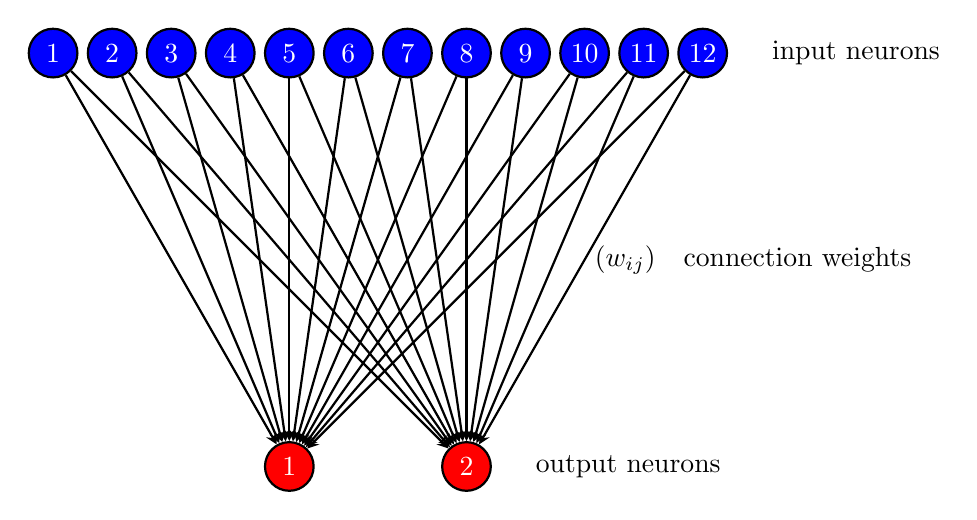
\begin{tikzpicture}[thick, scale=.75]
\node[circle, draw, fill=red, text=white] (O1) at (5, 0) {1};
\node[circle, draw, fill=red, text=white] (O2) at (8, 0) {2};
\foreach \i in {1, 2, ..., 12} {
	\node[circle, draw, fill=blue, label={center:\color{white}\i}] (I\i) at (\i, 7) {\phantom{0}};
	\draw[->, >=stealth] (I\i) -> (O1);
	\draw[->, >=stealth] (I\i) -> (O2);
}
\node[right] at (13,7) {input neurons};
\node[right] at (10, 3.5) {$\left( w_{ij} \right)$};
\node[right] at (11.5, 3.5) {connection weights};
\node[right] at (9,0) {output neurons};
\end{tikzpicture}
}
\end{center}
}

\frame[<+->]{\frametitle{Properties}
\begin{itemize}
	\item based on neural connections in the nervous system
	\item neurons are arranged in layers
	\item neurons outputs of one layer are connected to all neuron inputs of the subsequent layer
	\item connections are \emph{weighted}
	\item network functionality depends on:
	\begin{itemize}
		\item network topology
		\item connection weights
	\end{itemize}
\end{itemize}
}

\frame[<+->]{\frametitle{One neuron}
\begin{center}
\resizebox{0.8\textwidth}{!}{
\large
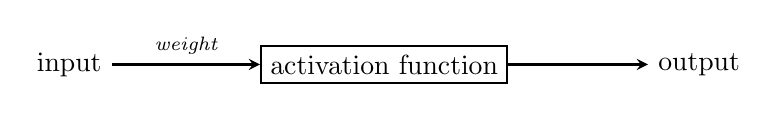
\begin{tikzpicture}[thick]
\node (a) at (0, 0) {input};
\node[rectangle, draw, align=center] (b) at (4, 0) {activation function};
\node (c) at (8, 0) {output};

\draw[->, >=stealth] (a) -> (b) node[midway, above] {\it \scriptsize weight};
\draw[->, >=stealth] (b) -> (c);
\end{tikzpicture}
}\\[2ex]\pause
Used activation function (sigmoid function):\\[1ex]
\resizebox{0.8\textwidth}{!}{
\begin{tikzpicture}[domain=-2.2:2.2, smooth, samples=50, >=stealth, scale=2, thick]

\draw[color=blue] plot (\x,{1 / (1+exp(- 4 *\x))}) node at (2.5, 0.7) {};

% Koordinatenachsen
\draw[->] (-2.2,0) -- (2.2,0) node[right] {$x$};
\draw[->] (0,-0.2) -- (0,1.2) node[above] {$f(x) = \dfrac{1}{1+e^{-ax}}$};
\draw (-0.05,1) --(0.05,1) node [left] {$1~$};
\draw (-0.05,0.5) -- (0.05,0.5) node [left] {$0.5~$};
\foreach \i in {-2, -1, 1, 2}{
	\draw (\i, -0.05) -- (\i, 0.05) node [below=1ex] {$\i$};
}
\end{tikzpicture}
}
\end{center}
}



\frame[<+->]{\frametitle{One neuron}
Neuron output depends on:\pause
\begin{enumerate}
	\item output of previous neurons
	\item connection weights
	\item activation function
\end{enumerate}
\begin{center}
\visible<+>{\emph{In the following experiment, S-Bot controllers only differ in (2).}}
\end{center}
}



\subsection{Artificial evolution}
\frame{\tableofcontents[currentsection, currentsubsection]}

\frame[<+->]{\frametitle{Abstract}
\begin{itemize}
	\item also based on biology
	\item uses \emph{selection, reproduction} and \emph{mutation}
	\item optimizes on the basis of a given \emph{fitness function}
	\item process:
	\begin{enumerate}
		\item create initial population
		\item calculate the fitness of each individual in the current population
		\item select a certain amount of well-fit individuals for reproduction
		\item breed next generation using reproduction and mutation
		\item repeat 2-4
	\end{enumerate}
\end{itemize}
%\visible<+->{Here: individuals represent weight matrices of the neural networks used as controllers.}
}


\frame{\frametitle{Example}
	\begin{block}{Initialization}
	\vspace{2ex}
	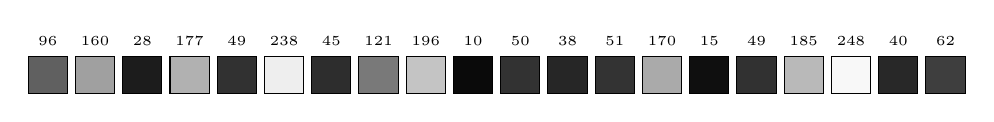
\begin{tikzpicture}[scale=0.6]
		\def\grayscales{{96, 160, 28, 177, 49, 238, 45, 121, 196, 10, 50, 38, 51, 170, 15, 49, 185, 248, 40, 62}}
		\foreach \i in {0, 1, ..., 19} {
			\pgfmathparse{array(\grayscales,\i)}
			\definecolor{gray\i}{RGB}{\pgfmathresult,\pgfmathresult,\pgfmathresult}
			\node[draw, fill=gray\i, label=above:{\tiny \pgfmathresult}] at (\i,0) {\phantom{A}};
		}
	\end{tikzpicture}
	\end{block}
}

\frame{\frametitle{Example}
	\begin{block}{Ordered by fitness}
	\vspace{2ex}
	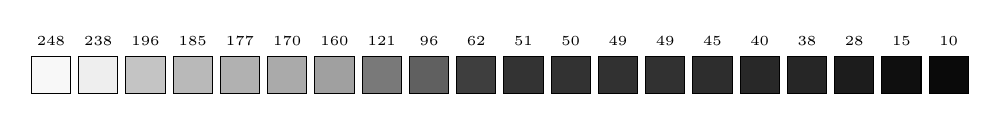
\begin{tikzpicture}[scale=0.6]
		\def\grayscales{{10, 15, 28, 38, 40, 45, 49, 49, 50, 51, 62, 96, 121, 160, 170, 177, 185, 196, 238, 248}}
		\foreach \i in {0, 1, ..., 19} {
			\pgfmathparse{array(\grayscales,19-\i)}
			\definecolor{gray\i}{RGB}{\pgfmathresult,\pgfmathresult,\pgfmathresult}
			\node[draw, fill=gray\i, label=above:{\tiny \pgfmathresult}] at (\i,0) {\phantom{A}};
		}
	\end{tikzpicture}
	\end{block}
}

\frame{\frametitle{Example}
	\begin{block}{Selection}
	\vspace{2ex}
	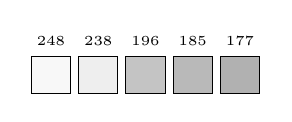
\begin{tikzpicture}[scale=0.6]
		\def\grayscales{{177, 185, 196, 238, 248}}
		\foreach \i in {0, 1, ..., 4} {
			\pgfmathparse{array(\grayscales,4-\i)}
			\definecolor{gray\i}{RGB}{\pgfmathresult,\pgfmathresult,\pgfmathresult}
			\node[draw, fill=gray\i, label=above:{\tiny \pgfmathresult}] at (\i,0) {\phantom{A}};
		}
	\end{tikzpicture}
	\end{block}
}

\frame{\frametitle{Example}
	\begin{block}{Reproduction}
	\vspace{2ex}
	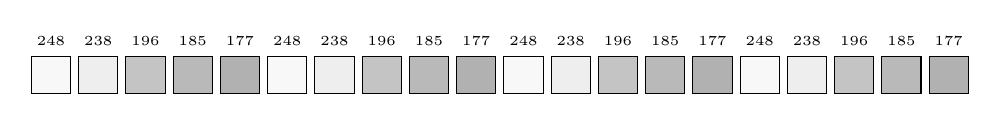
\begin{tikzpicture}[scale=0.6]
		\def\grayscales{{177, 185, 196, 238, 248, 177, 185, 196, 238, 248, 177, 185, 196, 238, 248, 177, 185, 196, 238, 248}}
		\foreach \i in {0, 1, ..., 19} {
			\pgfmathparse{array(\grayscales,19-\i)}
			\definecolor{gray\i}{RGB}{\pgfmathresult,\pgfmathresult,\pgfmathresult}
			\node[draw, fill=gray\i, label=above:{\tiny \pgfmathresult}] at (\i,0) {\phantom{A}};
		}
	\end{tikzpicture}
	\end{block}
}

\frame{\frametitle{Example}
	\begin{block}{Mutation}
	\vspace{2ex}
	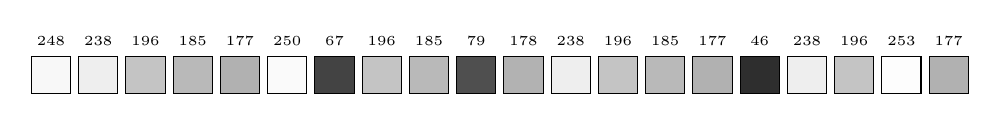
\begin{tikzpicture}[scale=0.6]
		\def\grayscales{{177, 253, 196, 238, 46, 177, 185, 196, 238, 178, 79, 185, 196, 67, 250, 177, 185, 196, 238, 248}}
		\foreach \i in {0, 1, ..., 19} {
			\pgfmathparse{array(\grayscales,19-\i)}
			\definecolor{gray\i}{RGB}{\pgfmathresult,\pgfmathresult,\pgfmathresult}
			\node[draw, fill=gray\i, label=above:{\tiny \pgfmathresult}] at (\i,0) {\phantom{A}};
		}
	\end{tikzpicture}
	\end{block}
}

\frame{\frametitle{Example}
	\begin{block}{Ordered by fitness again}
	\vspace{2ex}
	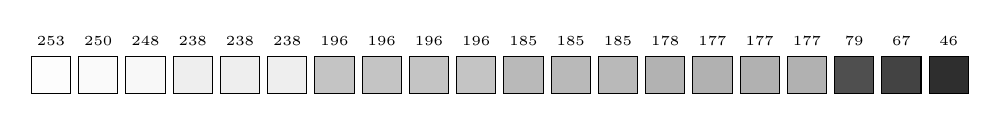
\begin{tikzpicture}[scale=0.6]
		\def\grayscales{{46, 67, 79, 177, 177, 177, 178, 185, 185, 185, 196, 196, 196, 196, 238, 238, 238, 248, 250, 253}}
		\foreach \i in {0, 1, ..., 19} {
			\pgfmathparse{array(\grayscales,19-\i)}
			\definecolor{gray\i}{RGB}{\pgfmathresult,\pgfmathresult,\pgfmathresult}
			\node[draw, fill=gray\i, label=above:{\tiny \pgfmathresult}] at (\i,0) {\phantom{A}};
		}
	\end{tikzpicture}
	\end{block}
}


\section{Experiment}
\frame{\tableofcontents[currentsection, currentsubsection]}

\frame{\frametitle{Process}
\only<1-3,5->{
\begin{block}{Five steps:}\pause
\begin{enumerate}
	\item<2-> The real robot is defined, including real hardware.
	\item<3-> A simulator is developed which can model the robot at different detail levels.
	\item<5-> A simplified model is chosen, that permits to run evolutionary experiments in a reasonable amount of time.
	\item<6-> Successful controllers from step 3 are improved using a detailed model.
	\item<7-> Successful controllers from step 4 are improved on the real hardware.
\end{enumerate}
\visible<8->{Here: only 1-3.}
\end{block}
}
\ifnum\handout=0
	\only<4>{
	\begin{center}
	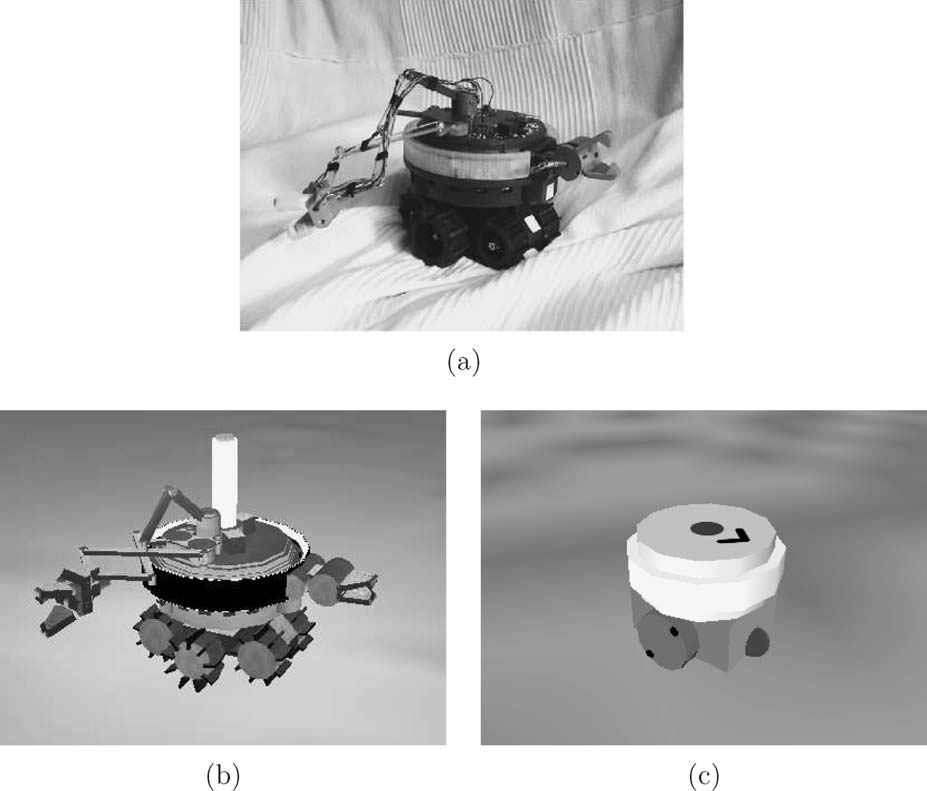
\includegraphics[
			width=0.55\textwidth,
		]{pics/sbot_sim_models.jpg}
	\end{center}
	}
\fi
}

\subsection{Aggregation}
\frame{\tableofcontents[currentsection, currentsubsection]}

\frame[<+->]{\frametitle{Setup}
\begin{itemize}
	\item simplified simulation model used, no turret, no grippers
	\item basically just a set of wheels with a speaker
	\item the speaker always emits a sound, which can be sensed by other S-Bots using three sound sensors up to a distance of 75~cm
	\item detection of neighbors or objects is done using 8 proximity sensors
	\item noise is simulated by a uniformly distributed random signal within $\pm 5\%$ of the sensors saturation value
	\item global area is $3\times 3$ meters, bigger than the perceptual range of the S-Bots
\end{itemize}
}

\frame[<+->]{\frametitle{Network structure}
\begin{center}
\resizebox{!}{0.82\textheight}{
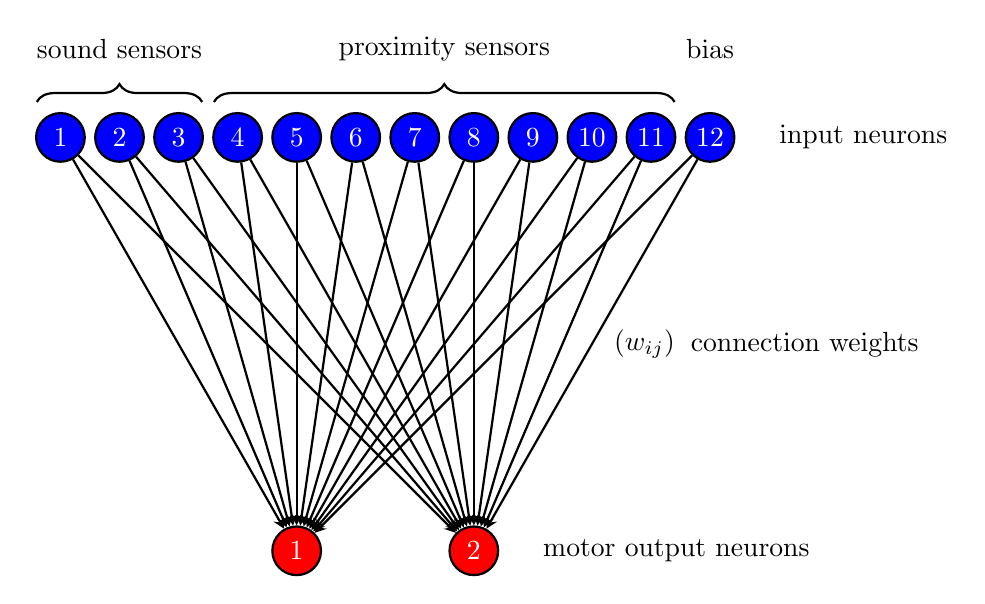
\begin{tikzpicture}[thick, scale=.75]
\node[circle, draw, fill=red, text=white] (O1) at (5, 0) {1};
\node[circle, draw, fill=red, text=white] (O2) at (8, 0) {2};
\foreach \i in {1, 2, ..., 12} {
	\node[circle, draw, fill=blue, label={center:\color{white}\i}] (I\i) at (\i, 7) {\phantom{0}};
	\draw[->, >=stealth] (I\i) -> (O1);
	\draw[->, >=stealth] (I\i) -> (O2);
}

\draw[brc] (0.6, 7.6) -- (3.4, 7.6) node at (2, 8.5) {sound sensors};
\draw[brc] (3.6, 7.6) -- (11.4, 7.6) node at (7.5, 8.5) {proximity sensors};
\node at (12, 8.5) {bias};

\node[right] at (13,7) {input neurons};
\node[right] at (10.2, 3.5) {$\left( w_{ij} \right)$};
\node[right] at (11.5, 3.5) {connection weights};
\node[right] at (9,0) {motor output neurons};
\end{tikzpicture}
}
\end{center}
}

\frame[<+->]{\frametitle{The evolutionary algorithm}
\begin{itemize}
	\item weights range in [-10, +10] and are represented by 8 bits
	\item each genotype consists of (12x2) x 8 = 192 bits.

	\item start with 100 random genotypes. Each is tested over 8 epochs
	\item one epoch means: random number, positions and orientation of sbots
	\item the top 20 genotypes produce 5 offsprings (flipping bits)
	\item each evolutionary run lasts 100 generations
	\item tested for 20 evolutionary runs

%	\begin{itemize}
%		\item each epoch represents 90 sec
%		\item each genotypes gets tested for 720 sec = 12 min
%		\item each generation of 100 genotypes takes 1200 min = 20 h
%		\item each evolutionary run of 100 generations takes 2000 h (83d)
%	\end{itemize}
\end{itemize}
}

\frame[<+->]{\frametitle{The evolutionary algorithm}
\begin{itemize}
	\item fitness function accounts for number of S-Bots used
	\item fitness of a genotype is the average fitness of all epochs
	\item genotype is evaluated for its aggregation and motion quality:
	\begin{itemize}
		\item does the genotype minimize the distance between sbot and the center of the group?
		\item do the wheels of the sbot turn in the same direction?
	\end{itemize}
\end{itemize}
}

\frame[<+->]{\frametitle{The evolutionary algorithm}
	\begin{center}
	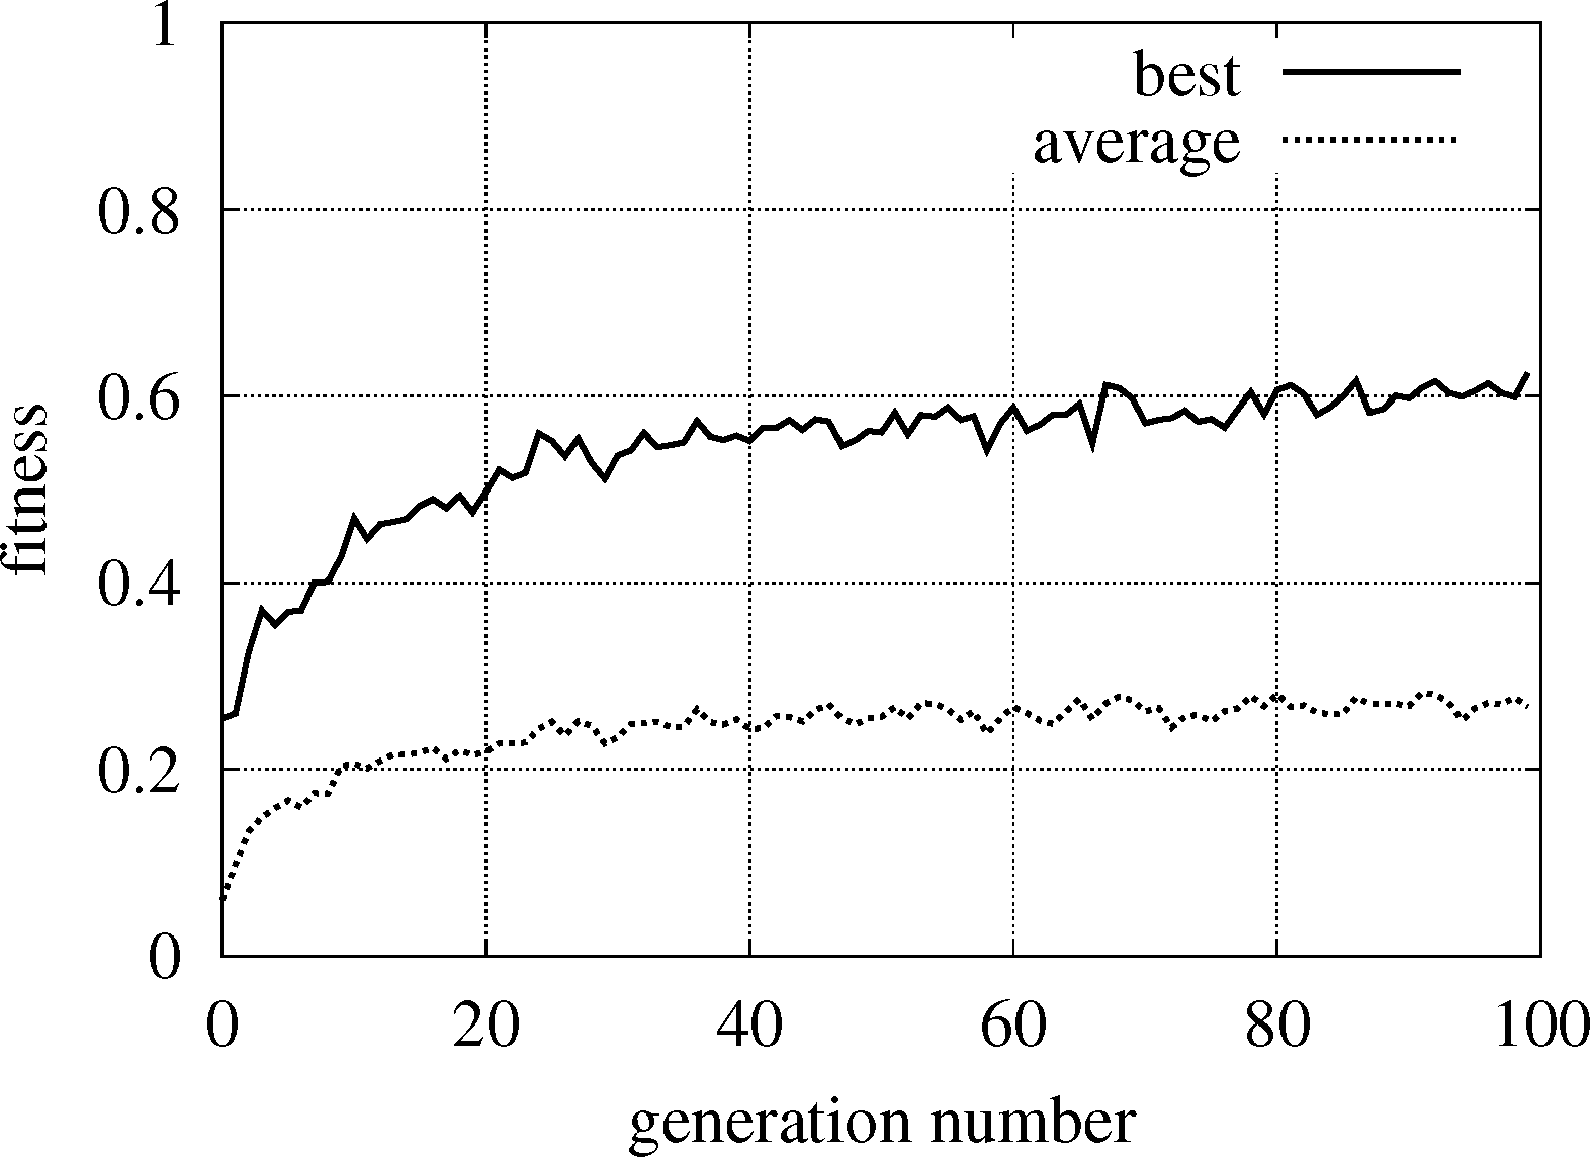
\includegraphics[
			width=0.55\textwidth,
		]{pics/03.png}
	\end{center}
	\begin{itemize}
		\item Aggregation perfomance averaged over 20 evolutionary runs
	\end{itemize}
\begin{center}
%\visible<+->{$\Rightarrow$Evolution with a time limit only delivers an estimate of the ''best'' genotype}
\end{center}
}

\frame[<+->]{\frametitle{Observations}
%\begin{itemize}
%	\item solitary S-Bots move in large circles, turning away from obstacles
%	\item differ mostly when s-bosts are close together, since then each strategy has its own balance between attraction of other S-Bots via sound recognized by sound senesors and repulsion of objects detected by proximity sensors
%
%\end{itemize}
	\begin{center}
	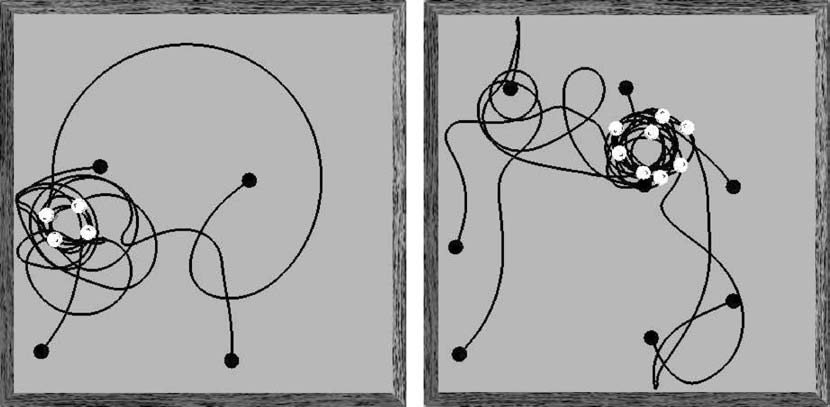
\includegraphics[
			width=0.6\textwidth,
		]{pics/04.png}
	\end{center}
	\begin{itemize}
		\item Aggregation behavior.\\Following behavior of small groups emerges, if the group size gets larger, chaos increases.
	\end{itemize}
}


\frame[<+->]{\frametitle{Scalability}
%\begin{itemize}
%	\item tested with 4-40 S-Bots
%	\item new measure for aggregation quality, using new minimal radius approximation
%	\item about half of the tested controllers showed acceptable aggregation quality
%	\item the best showed a behavior, where the aggregate moved slowly around the area
%\end{itemize}
	\begin{center}
	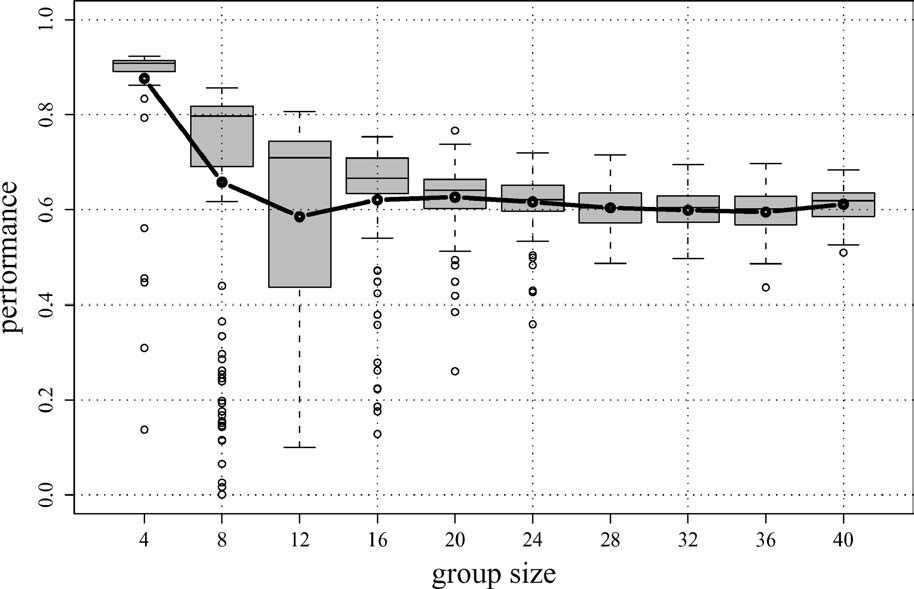
\includegraphics[
			width=0.65\textwidth,
		]{pics/06.png}
	\end{center}
	\vspace{-1ex}
	\begin{itemize}
		\item Best genotype of each run tested against increasing group sizes.
	\end{itemize}
}


\subsection{Coordinated motion}
\frame{\tableofcontents[currentsection, currentsubsection]}

\frame[<+->]{\frametitle{Coordinated motion}
	\begin{center}
		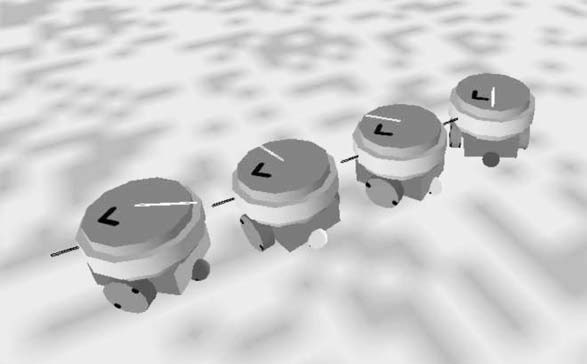
\includegraphics[width=0.5\textwidth]{pics/07.png}
	\end{center}
\begin{itemize}
	\item problem: S-Bot start with different orientations
	\item try to solve this problem and to evolve coordinated movement using only local information
\end{itemize}
}


\frame[<+->]{\frametitle{Simulation}
\begin{itemize}
	\item no sound, S-Bots already connected via rigid links representing the grippers
	\item each S-Bot now has:
	\begin{itemize}
		\item a turret that can rotate with respect to its chassis
		\item a traction sensor indicating the angle between its turret and the chassis and the force of the traction
	\end{itemize}

\end{itemize}
}

\frame[<+->]{\frametitle{Simulation}
	\begin{center}
	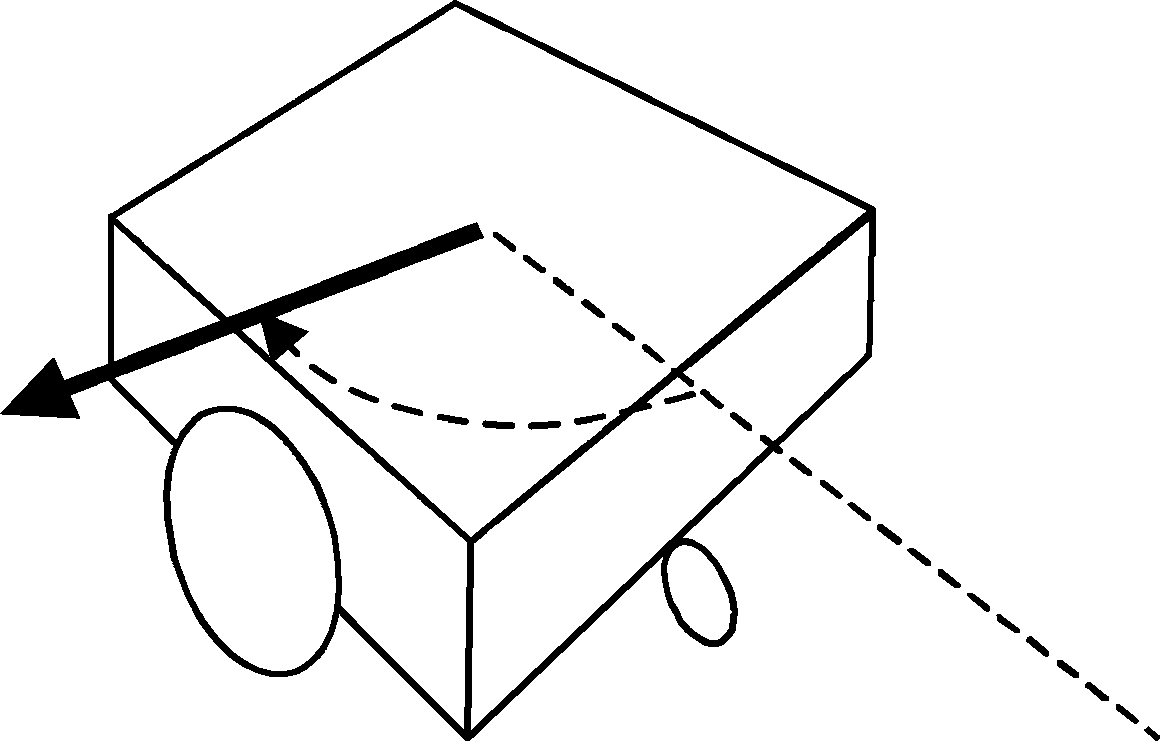
\includegraphics[
			width=0.45\textwidth,
		]{pics/08.png}
	\end{center}
	\begin{itemize}
		\item traction sensor provides an average direction towards which the group is trying to move as a whole
		\item measure the mismatch between the group's direction and the S-Bot's chassis direction
	\end{itemize}
}

%\frame[<+->]{\frametitle{The evolutionary algorithm}
%\begin{itemize}
%	\item S-Bot controller is a neural network: 4+(1 bias) input neurons, 2 output neurons
%	\item the 4 inputs encode the intensity of the traction from the 4 different directions: front, right, back and left
%	\item if the difference between a sensors preferred direction and the traction angle is in $[-90^\circ, +90^\circ]$ it scales the cosine of that angle difference with the traction force so that it can then be mapped to wheel speeds in the direction of that sensor
%	\item same evolution as in aggregation except one genotype is now just $8 \times (5 \times 2) = 80$ bit
%	\item fitness of an epoch is the Euclidean distance between the center of the group at the beginning and at the end of the epoch
%\end{itemize}
%}

\frame[<+->]{\frametitle{Network structure}
\begin{center}
\resizebox{!}{0.7\textheight}{
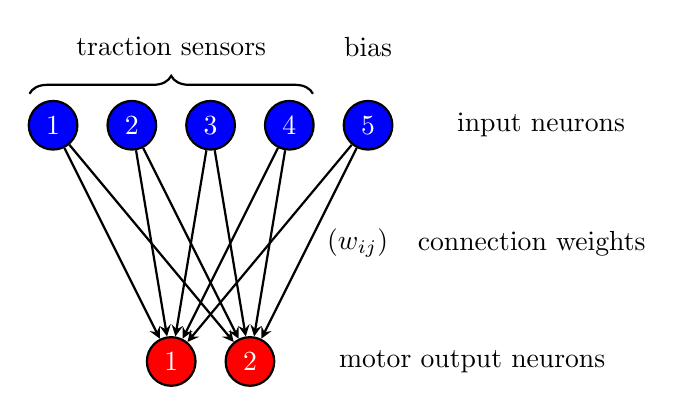
\begin{tikzpicture}[thick, scale=1]
\node[circle, draw, fill=red, text=white] (O1) at (2.5, 0) {1};
\node[circle, draw, fill=red, text=white] (O2) at (3.5, 0) {2};
\foreach \i in {1, 2, ..., 5} {
	\node[circle, draw, fill=blue, label={center:\color{white}\i}] (I\i) at (\i, 3) {\phantom{0}};
	\draw[->, >=stealth] (I\i) -> (O1);
	\draw[->, >=stealth] (I\i) -> (O2);
}

\draw[brc] (0.7, 3.4) -- (4.3, 3.4) node at (2.5, 4) {traction sensors};
\node at (5, 4) {bias};

\node[right] at (6,3) {input neurons};
\node[right] at (4.35, 1.5) {$\left( w_{ij} \right)$};
\node[right] at (5.5, 1.5) {connection weights};
\node[right] at (4.5,0) {motor output neurons};
\end{tikzpicture}
}
\end{center}
}

\frame[<+->]{\frametitle{The evolutionary algorithm}
\begin{itemize}
	\item sensor inputs is the cosine of the angle diff' between each sensor's prefered direction and the group traction
	\item evolution basically the same as used with aggregation
	\item measure the fitness for each epoche as the Euclidean distance between start and endpoint of the group
\end{itemize}
}

\frame[<+->]{\frametitle{The evolutionary algorithm}
\begin{center}
	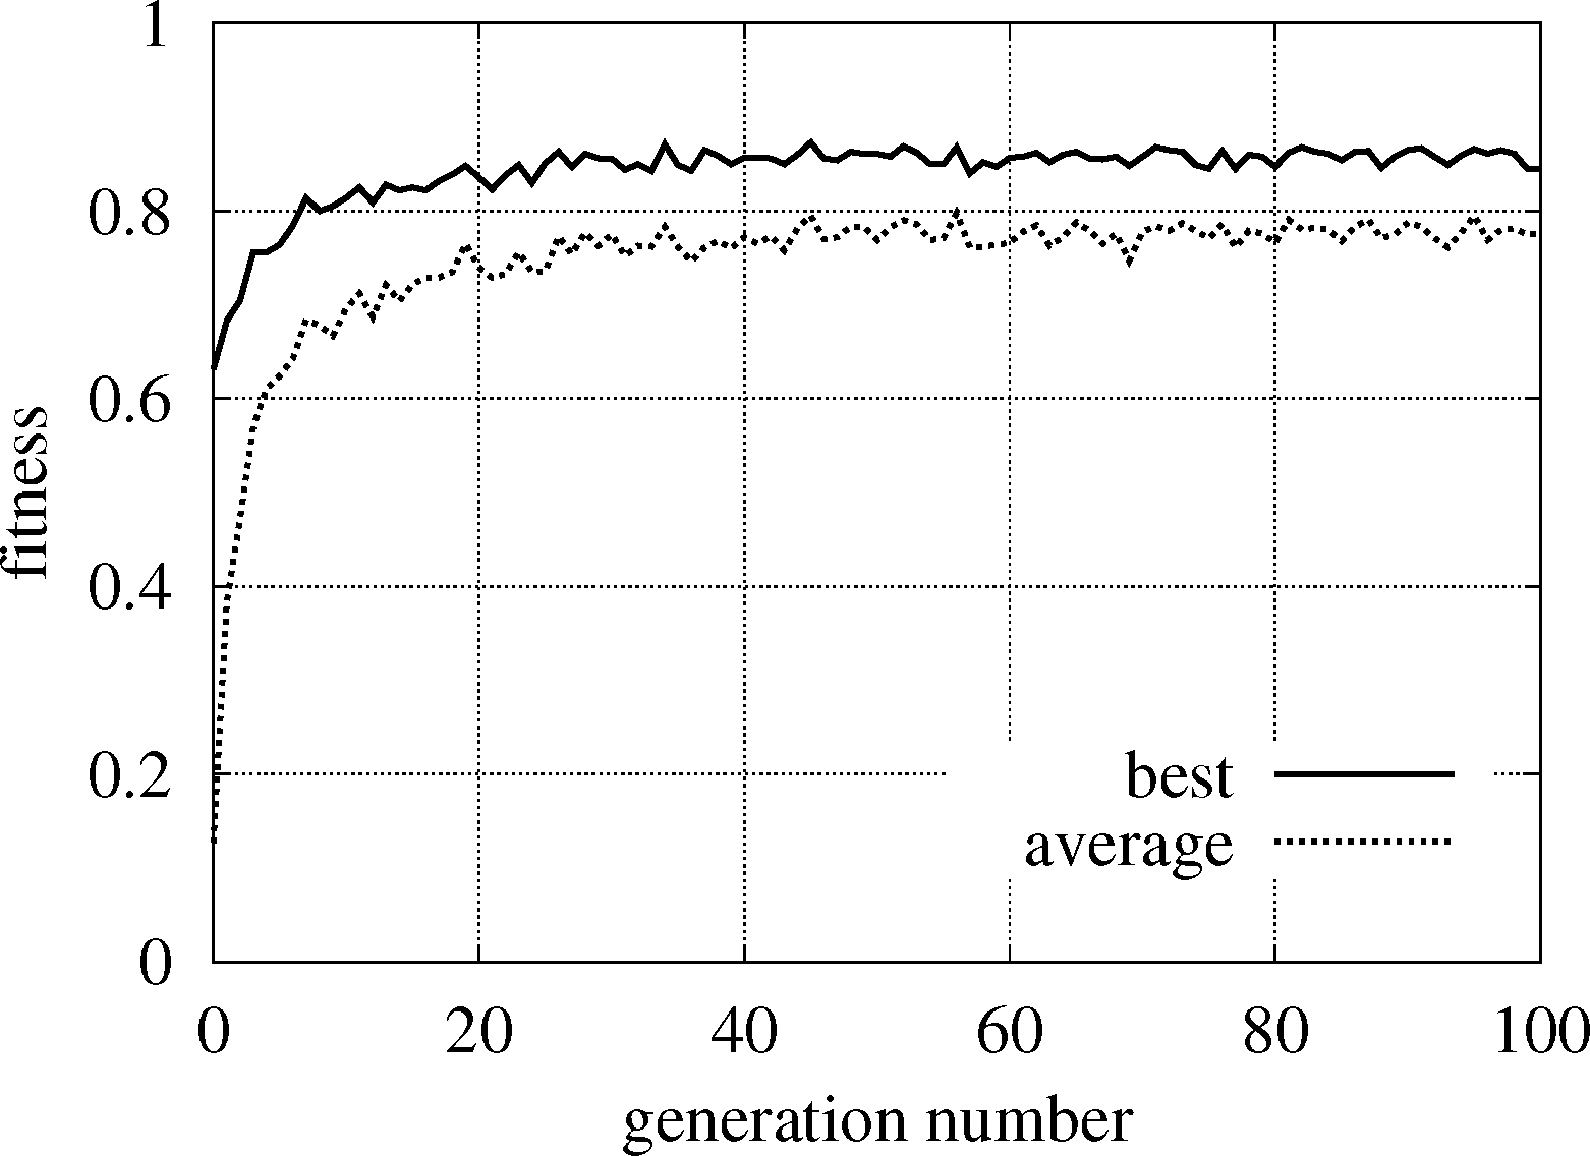
\includegraphics[
			width=0.55\textwidth,
		]{pics/09.png}
\end{center}
\begin{itemize}
	\item Coordinated movement performance for 20 runs à 100 generations.
\end{itemize}
}


\frame[<+->]{\frametitle{Observed behavior}
\begin{itemize}
	\item each S-Bot makes a move in "its" direction
	\item thereby each S-Bot receives a traction direction in correspondence to the majority of orientations among the group
	\item evolved controller pattern:
	\begin{itemize}
		\item if orientation is almost identical, traction is near 0, everyone just continues full speed
		\item if traction is low, each bot tweaks a bit in the average direction
		\item if traction is high and orientation is highly misaligned then the S-Bots with higher difference change their orientation more rapidly than the ones who receive a higher traction
	\end{itemize}
	\item side effects: object avoidance and object pulling
\end{itemize}
}


\frame[<+->]{\frametitle{Scalability}
%\begin{itemize}
%	\item still works with different number of S-Bots, different rigid formations and even with flexible links
%	\item when links are flexible, the formation changes in the beginning because of the different spawning orientations but then settles for a stable formation
%	\item tested with group sizes in the pattern $4, 8, 12, \dots, 40$
%	\item when group size increases, more time is needed to negotiate a common direction
%	\item extreme cases are, when the group needs all the experiment time to negotiate a direction or when the group revolves around its center
%	\item smaller groups revolve more often, because it is more likely that the S-Bot spawn with orientations that favor this behavior
%\end{itemize}
	\begin{center}
	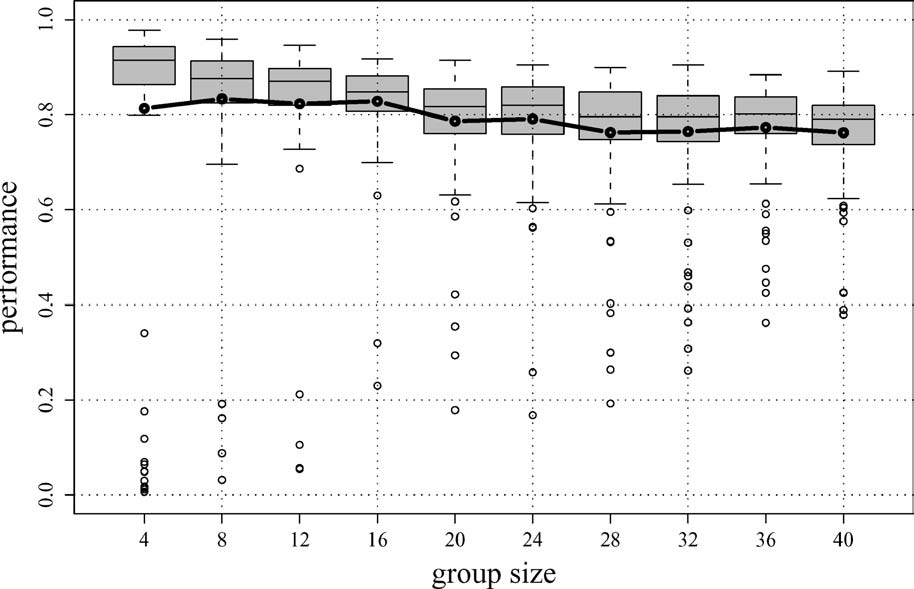
\includegraphics[
			width=0.65\textwidth,
		]{pics/15.png}
	\end{center}
	\vspace{-1ex}
	\begin{itemize}
		\item Coordinated movement performance for increasing group sizes.
	\end{itemize}
}

%\frame[<+->]{\frametitle{Obstacle avoidance}
%\begin{itemize}
%	\item when a S-Bot hits an obstacle, the collision creates a force in the opposite direction which is received by the S-Bot as a traction force
%	\item to cancel this traction the S-Bot changes its orientation thereby avoiding being stuck
%	\item when this S-Bot is connected with other S-Bot the collision traction is received by the whole group and therefore the groups tries to cancel the traction, avoiding the obstacle
%\end{itemize}
%}

%\frame[<+->]{\frametitle{Object pulling}
%\begin{itemize}
%	\item S-Bot connected to an object tend to push/pull this object in a coordinated fashion
%	\item can be explained by the fact that evolved controllers do try to follow the average group direction but also have a tendency to maintain their own direction if they receive a low traction from an angle close to $180^\circ$ which in a normal scenario would be some S-Bot still misaligned to the group's direction
%\end{itemize}
%}

\section{Validation using the realistic model}
\frame{\tableofcontents[currentsection]}

\frame[<+->]{\frametitle{Detailed Model}
%\begin{itemize}
%	\item realistic model experiments use the same setup, same evolution, same group sizes etc.
%	\item aggregation process is slower, because the tracks on the wheels slow their movement/responsiveness and therefore limits the following behavior which limits the performance of lower group sizes
%	\item coordinated movement is surprisingly comparable
%	\item limiting factor again is the lesser responsiveness when it comes to movement abilities
%	\item taking more time to turn their chassis means a longer coordination phase and leaves less time for the movement phase
%\end{itemize}
	\begin{center}
	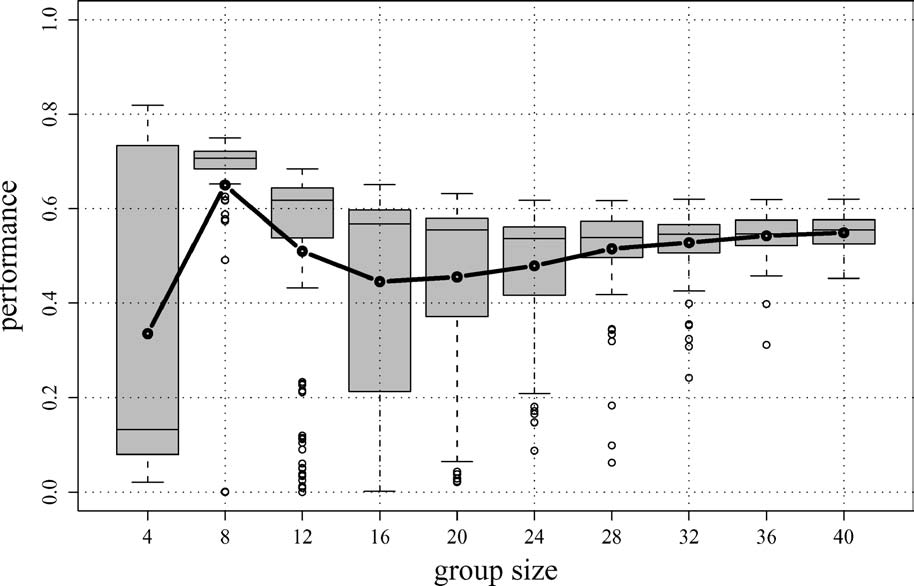
\includegraphics[
			width=0.65\textwidth,
		]{pics/16.png}
	\end{center}
	\vspace{-1ex}
	\begin{itemize}
		\item Aggregation performance for increasing group sizes (detailed model)
	\end{itemize}
}


\section{Summary}
\frame{\tableofcontents[currentsection]}
\frame[<+->]{\frametitle{Summary}
\begin{itemize}
	\item multi-stage evolution possible, using the simplified model first to find a suitable solution then continue from there with a detailed model
	\item Drawbacks:
	\begin{itemize}
		\item the evaluation functions used in this simulation used global information (position of each S-Bot etc.)
		\item to evolve these controllers on real hardware evaluation needs to be performed using only local available information
		\item could be bypassed by using a camera in a real setup to obtain positions
	\end{itemize}
\end{itemize}
}


\end{document}

